\section{Process' Perspective}

\subsection{Collaborative Development \& Team Organization}

When we initially talked about teaming up we made sure to align our expectations. We agreed that each member expected to spend 8-12 hours a week on the course. Thus our way of working became something like this:
\begin{itemize}
    \item Tuesday, 10-14: Project Work
    \item Tuesday, 14-16: Lecture
    \item Tuesday, 16-18: Exercises/Project Work
    \item Friday, 10-15: Project Work (When possible, not each Friday)
\end{itemize}

The above points were all physically present sessions for all members. Each member had the freedom to do additional work at other times during the week. All communication was through a Discord channel.

When working, we would at times do versions of pair programming. Teamwork was however difficult, since all concepts were new to everybody, and a lot of the understanding and progress came from trial and error. All sessions were an open forum where questions were welcome, and help was always possible to get. Sadly, we were not always good at remembering co-authorship on commits which might make the repository contributions look rather skewed.

We intended to utilize GitHub Issues to share the tasks between us, making sure not to be wasting time on duplicate work.


\subsection{CI/CD Chain}
%A complete description of stages and tools included in the CI/CD chains.
%That is, including deployment and release of your systems.
%- Github Workflows
%- Digital Ocean
% illustration af pipeline
% deployement and release
% hvilke ting kører vi hvornår og hvorfor


\begin{figure}[H]
    \centering
    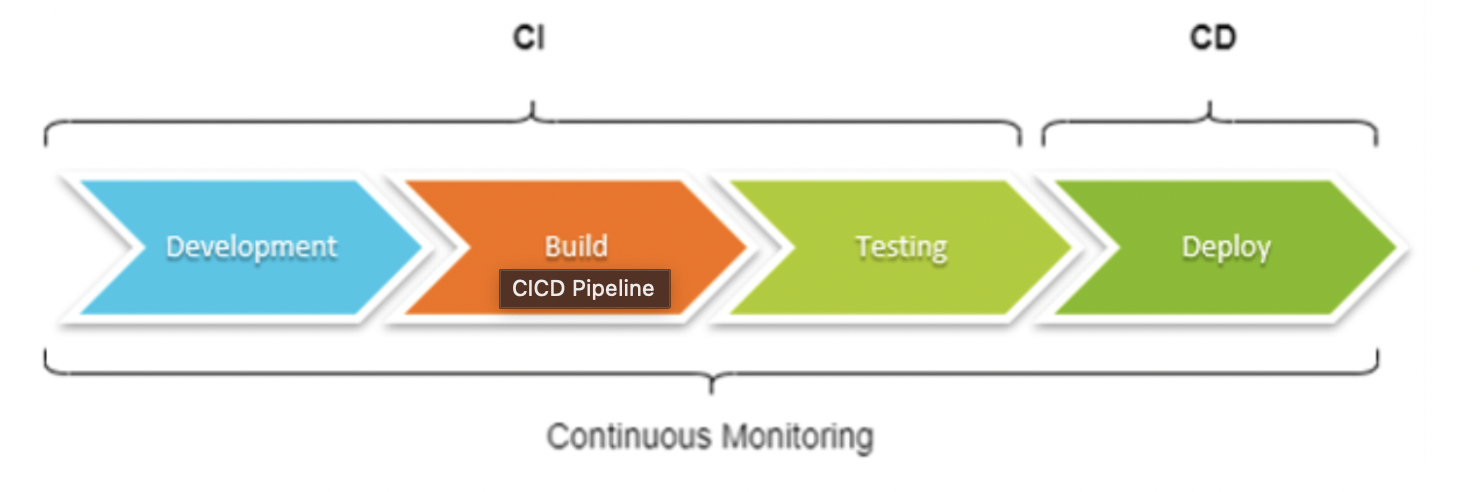
\includegraphics[width=0.65\linewidth]{Report/Images/CICD.png} 
    \caption{CI/CD pipeline}
    \label{fig:CICD}
\end{figure}


our CI/CD chain can be split into different stages. 
Developtment
- 
build
- 
testing
- 
deployment
- 

In our application, we have implemented a CI/CD chain by defining a handful of \texttt{.yml} files that utilize GitHub Actions. One of these files is responsible for the continuous deployment aspect of the pipeline. Through this workflow, we have automated the building, testing, and deployment process. Combined with the use of GitHub secrets, these workflows provide a powerful solution to automated deployment. Furthermore, it's a convenient way to manage our application's deployment process while maintaining confidentiality and flexibility. 
However, it does come with a drawback: Scalability is somewhat limited. This is because the workflow uses repository secrets to reference the Ip-addresses of our servers.
Had we been a company that wanted to change our Server-provider to something other than DigitalOcean, or simply looking to add more servers, we would have to add a separate paragraph to the workflow and update the repository secrets manually.
\newpage
\noindent The stages of our CD are as follows:

\begin{enumerate}
    \item Login to Docker Hub (using repository-secrets)
    \item Build and push minitwit-souffle
    \item Build and push minitwit-db
    \item Configure SSH (copying ssh-key)
    \item Deploy to Server (docker stop + rm old, pull and run new images)
    \item Copy docker-compose files to the server for Monitoring
    \item Running docker-compose files to start Monitoring
    \item Copy files for Logging and Deploy
    \item Running docker-compose files to start logging
\end{enumerate}

\noindent Additionally, we implemented an auto-release function to further streamline the deployment process, ensuring the latest code changes automatically are pushed to deployment. This was done by making a release each Sunday at 20:00 CEST. 

%%%%%%%%%%%%%%5---- asger tilføj noget her buddyboiiii


\subsection{Repository Organization \& Development Strategy}
\subsubsection{Repository Organization}

We structured our code in a mono-repository for two main reasons:
\begin{enumerate}
    \item It provides improved collaboration, as all developers are working on the same codebase.
    \item It simplifies version control as we only have a single history for all code.
\end{enumerate}
Another consideration was, that we didn't feel the need to divide it up, as the application is still relatively small. It would also add what we deemed to be unnecessary complexity by requiring different repositories to be cloud-hosted for cross-access since the necessary references in our C\# code would no longer reside in the same .NET solution.


\subsubsection{Development Strategy}

We utilized feature branching as our strategy as it has multiple advantages that work very well with the DevOps way of working. An example of this is continuous integration. The GitHub Actions make it simple to automate a require-to-pass test suite before any feature branch is merged into the main one. Other advantages include:

\begin{itemize}
    \item It isolates changes to specific features, minimizing conflicts with separate work.
    \item It facilitates the code review process that in turn ensures quality assurance.
    \item It provides a clear separation of work, which makes collaboration easier.
    \item It makes parallel development possible.
\end{itemize}

Our tasks were organized in GitHub Issues. This made it possible for each member to always be able to see which tasks were up for grabs, and who were working on what. It also acted as a task backlog giving an overview of the work that was yet to be done.

\noindent As the project progressed, however, the tasks began including the whole group, and the Issues board became slightly irrelevant.

\subsection{Monitoring \& Logging}
%How do you monitor your systems and what precisely do %you monitor?
%What do you log in your systems and how do you %aggregate logs?

\subsubsection{Monitoring} \label{Monitoring}

We monitor our system by having Prometheus gather metrics from our metric endpoints regularly. This is made possible by the NuGet package Prometheus.net, which is responsible for exposing a metrics endpoint in our API, which Prometheus can then send requests to. This data is then queried again by Grafana, which is responsible for visualizing it. We can access Grafana's dashboard through the user we set up. Our current metrics are:

\begin{itemize}
    \item Http-requests (Duration)
    \item Total Users
    \item Total Messages
    \item Average request duration (Last 2 minutes)
\end{itemize}

\noindent Together, these metrics provide information about how much stress we can expect our system to experience, and what kind of request intensity we can expect. It also provides an overview of user growth, giving us a sense of the direction our service is headed. 

Additionally, we are also making use of Digital Ocean to monitor our hardware such as the CPU and memory usage of our droplets.

\subsubsection{Logging} \label{Logging}

In order to log we are making use of the Serilog.Sinks.Elasticsearch NuGet Package. In our application, we have specified some metrics that ElasticSearch 

Kibana then retrieves the logging data from this sink and displays it.
We are logging all exceptions, requests to the controllers, and different functionalities happening in the middleware. 

skiftet default logger ud med serilog - andet format 
alle logs vi får er logs fra middleware 
default configuration logs - 


Log messages are generated to capture important events, errors, or relevant information during runtime. These logs are collected and forwarded to ElasticSearch, that then indexes and stores the data. Kibana then connects to ElasticSearch 

we use - sink direkte fra .NET direkte ind til (serilog - logging framework). en sink, der hvor alle logs glider hen. Den sink er sat til elastik search hvor kibana kan vise os logs på en pæn måde.
sender det videre til elastisearch direkte
det er kun logs fra .Net så vi kan formattere det her og fortælle hvad vi gerne vil logge og hvordan det skal se ud direkte i serilog. 
der er formartering i serverens programfil, men bliver måske ikke brugt ved deployment. 
triggers i middleware. når vi modtager request bliver der lavet en log, når den er færdig med at processe - værktøjer der laver logs for os. 

alle exceptions
request til controllers
masse andre ting der er I middleware - 


\subsection{Security Assessment}

Our security assessment consisted of a penetration test - Zed Attack Proxy, or ZAP, that showed some flaws in our program. Most seemed to be relatively simple to fix, and none seemed to be too severe in nature:
\begin{itemize}
    \item No Anti-CSRF tokens were found in a HTML submission form
    \item Passive (90022 - Application Error Disclosure)
    \item Content Security Policy (CSP) Header Not Set
    \item Missing Anti-clickjacking Header
    \item X-Content-Type-Options Header Missing
    \item Hidden File Found
    \item Vulnerable JS Library
    \item XSLT Injection might be possible.
    \item Cloud Metadata Potentially Exposed
\end{itemize}

\noindent These items resulted in GitHub Issues; some of which were dealt with while others were down-prioritized.

\subsection{Scaling \& Load Balancing}
%Applied strategy for scaling and load balancing. 

Our applied strategy for scaling and load-balancing, was implementing Docker Swarm for fault tolerance and replication, along with Nginx for load balancing working as a reverse proxy. This combination of Nginxs load balance capabilities and Docker Swarms dynamic scaling would result in an improvement of the systems overall availability and realiability. Hence in case of a system failure Nginx would redirect all load balance from one replica to another while docker swarms dynamically scaling would ensure that the system would be able to keep up with accelerating request and users. However, in our setup, we encountered some internal network delays that affected the system's performance, when Nginx was responsible for redirection. This resulted in Nginx not being fully implemented.

%------ nogen skal læse det her igennem _------
%loadbalancer: nginx, reverse proxy, 

%kinda docker-swarm 
%- nginx delay?
%- det var meningen at den skulle tage sig af redirection, men det virkede ikke som om at vi kunne det.
%- Det interne netværk skulle have tilladt redirection, men gjorde det ikke 

\subsection{AI Assistance}
%In case you have used AI assistants for writing code during your project or to write the report:
%Explain which system(s) you used during the project.
%Reflect on how it supported/hindered your process.
%In essence, it has to be clear how code or other artifacts come from ideas into the running system and everything that happens on the way.



\noindent As developers we have embraced the tool that is AI. We have used ChatGPT as a sparring partner whenever we got a task we did not know how to solve, or when we got stuck. It has been mostly great at providing ideas or starting points, but it has probably been at its best when troubleshooting or debugging. If nothing else it has provided the services of a rubber duck.

\noindent We have also used it in the formulation of documents like the SLA agreement, as it is mostly boilerplate text anyways. We provided it with some information about our system and what guarantees we could give, and it returned a rough draft we could finalize.

\noindent Finally, one team member has been using GitHub Copilot as an advanced intellisense tool, but not for making several lines of code. Meaning that it was used to finish individual lines of code, but not for making entire methods or blocks of code.